%%%% fs-run-time-experiments   Experiments

\label{fs-experiments-section}

\subsection{Setup}
We performed the series of experiments in order to estimate the performance of our system's prototype. As a stream processing task, we apply building an inverted index for Wikipedia documents. The computation of inverted index is implemented in terms of MapReduce transformations. We start with page mapping into the pairs {\it (word; word positions within the page)}. After that, word positions are reduced by word into the single structure. We assume the output of the stream to be change records of the inverted index structure, i.e. each input page triggers the output of the corresponding updates. 

Pairs {\it (word; word positions within the page)} must be ordered by page id and version before the update of inverted index state. Otherwise, it is possible to obtain the inconsistent index, if there are multiple versions of the same document.  
In the real-world, such scenario can be found in freshness-aware systems e.g. news processing engines. By the notion of {\it latency} we assume the time between two events: 
\begin{enumerate}
    \item Input page is taken into the stream
    \item All the change records for the page leave the stream
\end{enumerate}

In \FlameStream\ this algorithm is implemented as the typical conversion of MapReduce transformation, which is shown in section~\ref{fs-drifting}. Inverted index structure plays the role of an accumulator, and the accumulator map produces the most recent changes of this structure if any.

Our experiments were performed on the cluster of Amazon EC2 micro instances with 1GB RAM and 1 core CPU. We used 10000 Wikipedia articles as a dataset. 

\subsection{Overhead and scalability}

We take the ratio of arrived at the barrier items count to the number of the valid items among them as a key metric for the estimation of the overhead of our prototype. This value clearly represents the extra cost of our approach.

The relation between the number of workers, the delay between input documents and the proposed ratio is shown in Figure~\ref{overhead}. As expected, the peak of the ratio is achieved when the document per second rate is high, and the number of the nodes is low. This behavior can be explained by the fact that a few workers cannot effectively deal with such intensive load. Nevertheless, the proportion of invalid items reduces with the increase of workers number. Under non-extreme load, the total overhead of the optimistic approach is under 10\% for all considered number of workers. These results confirm that the ratio does not increase with the growth of the number of nodes.

\begin{figure}[htbp]
  \centering
  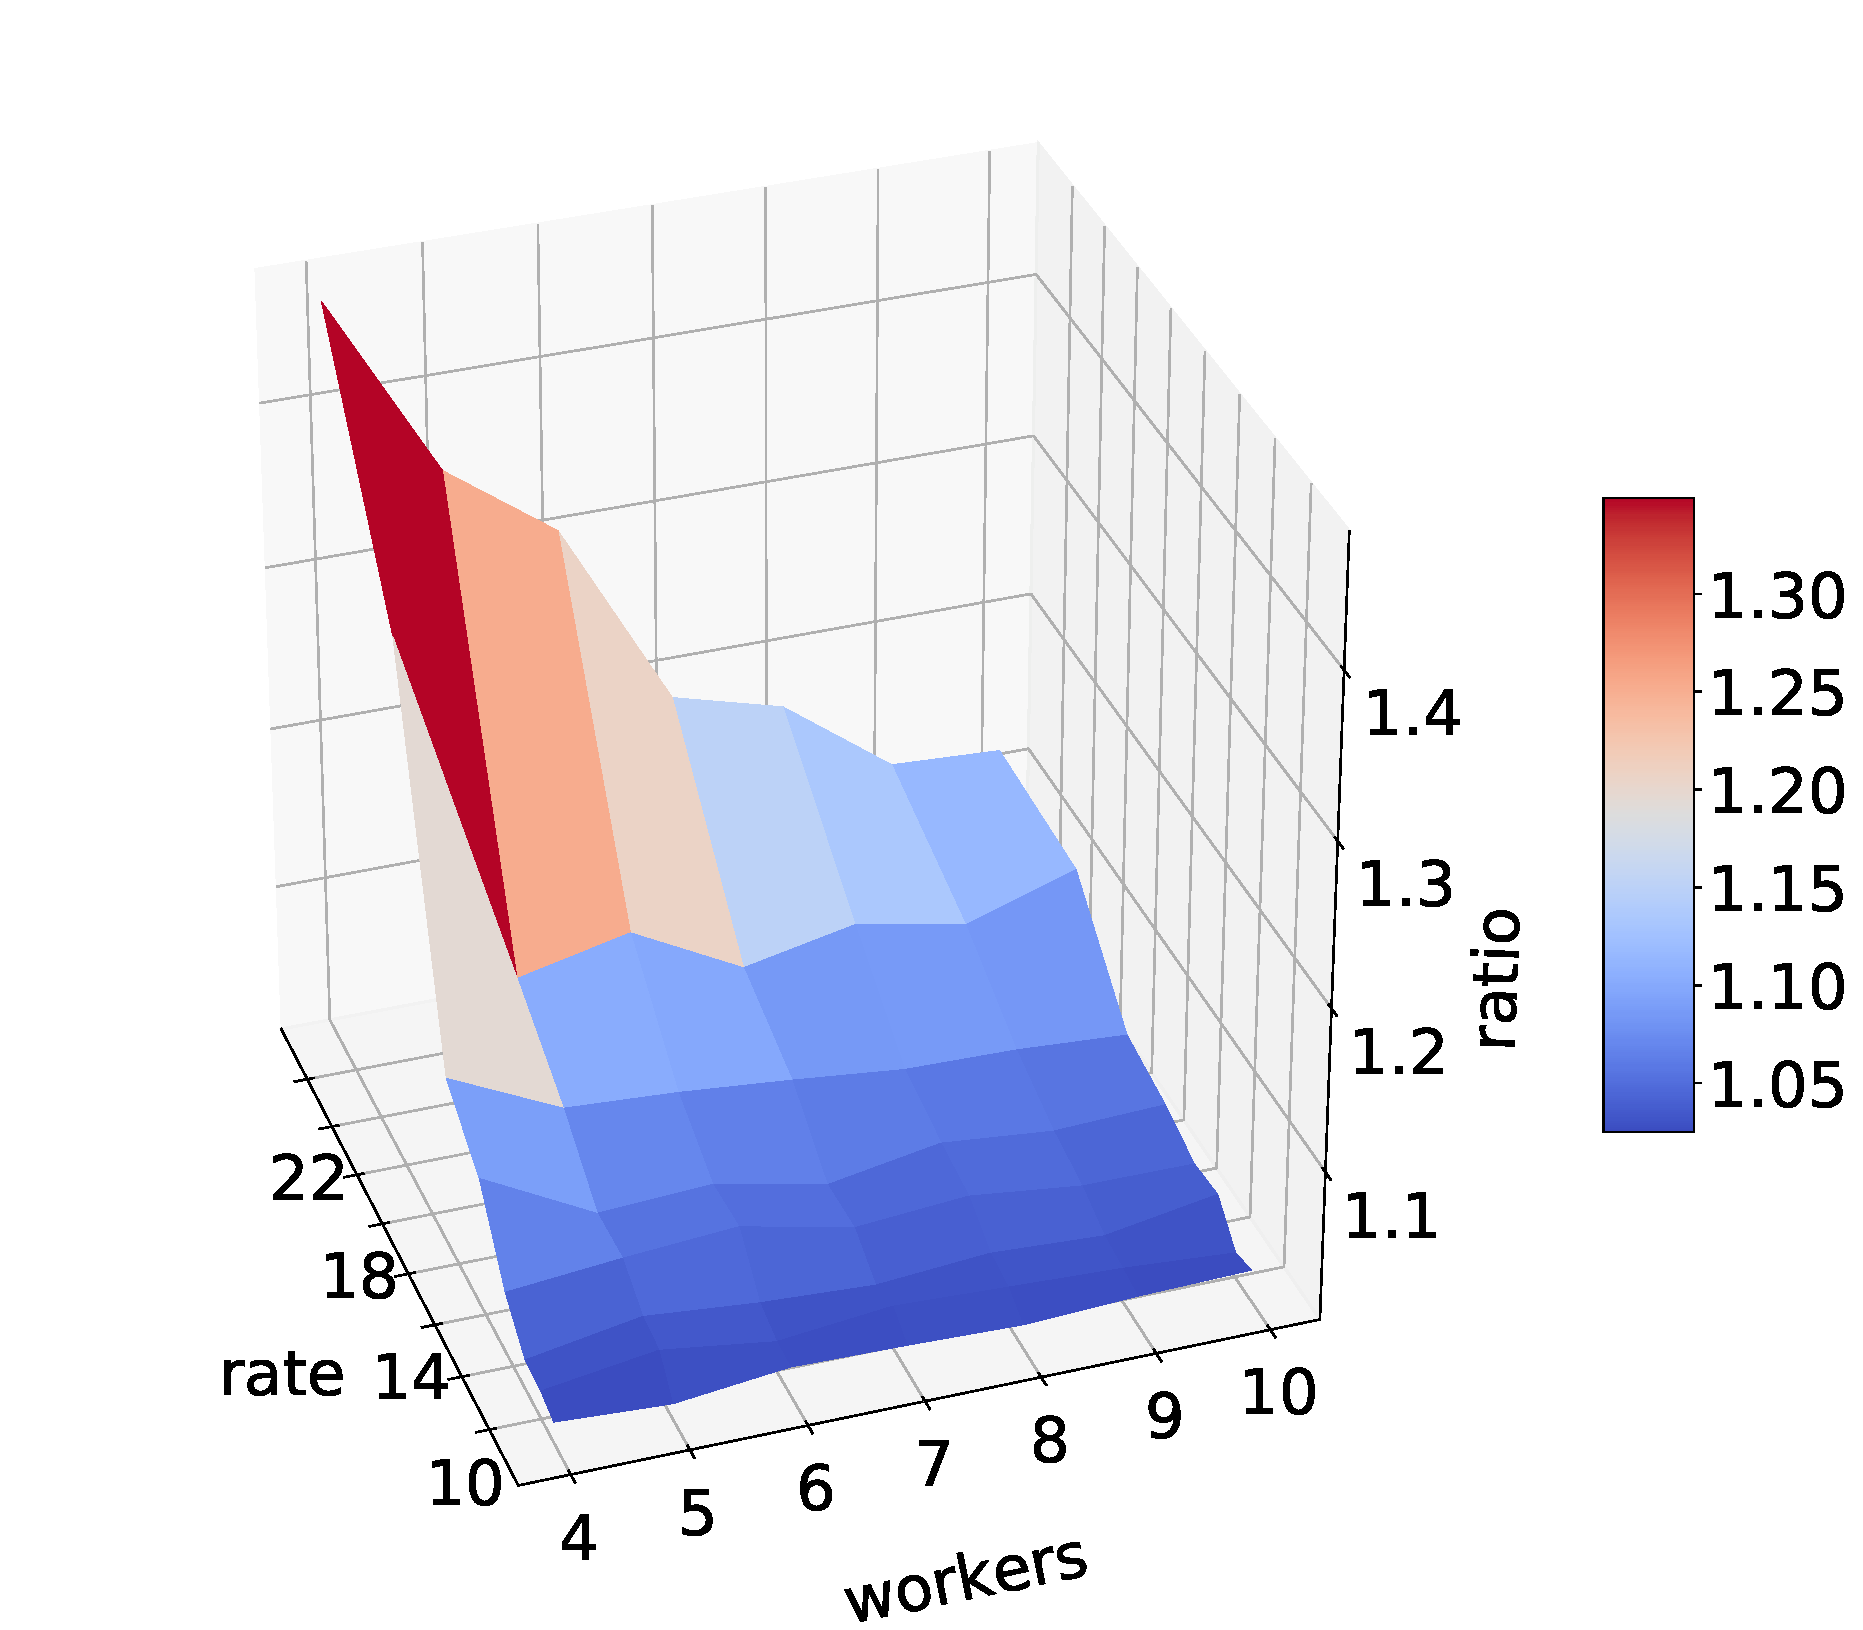
\includegraphics[width=0.5\textwidth]{pics/overhead}
  \caption{The relation between the number of workers, the delay between input documents and the replay ratio}
  \label {overhead}
\end{figure}

The latencies of \FlameStream\ across multiple workers for the fixed document rate of 70 ms are shown in Figure~\ref{fs-index-quantiles}. These figure demonstrate that latency is not significantly increased with the growth of the number of workers. 

Therefore, the most important conclusions of these experiments are: the proposed method is scalable, the overhead could be optimized by system setup.

\begin{figure}[htbp]
  \centering
  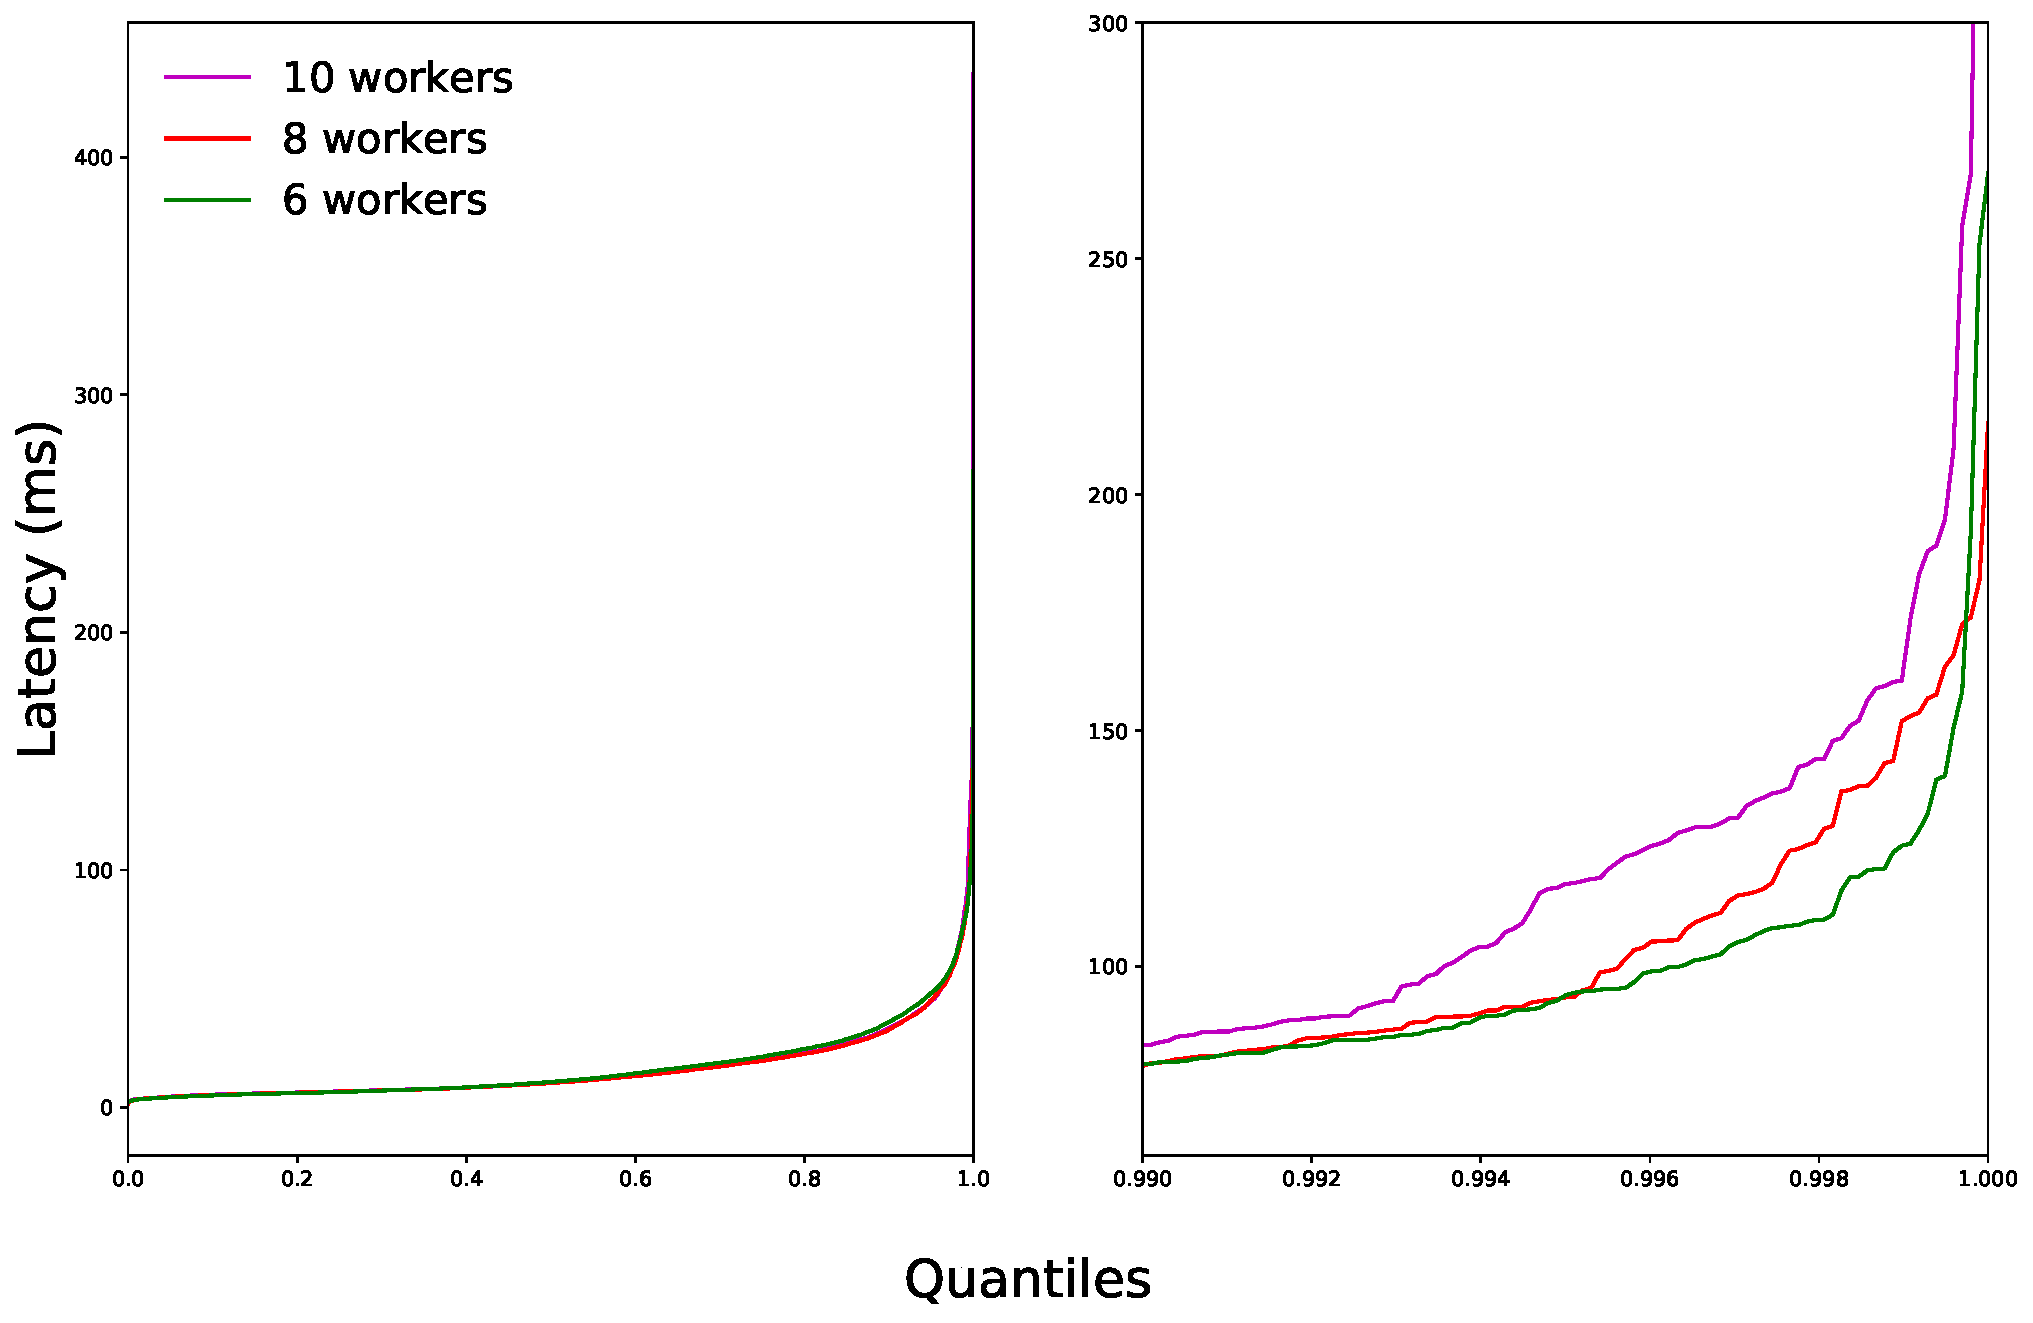
\includegraphics[width=0.48\textwidth]{pics/fs-index-quantiles}
  \caption{FlameStream latency distribution. Left - the whole distribution, right - tail latencies}
  \label {fs-index-quantiles}
\end{figure}

\subsection{Comparison against Apache Flink}

One of the most important goals of the experiments is the performance comparison with an industrial solution in terms of latency. Apache Flink is chosen for evaluation because it is state-of-the-art stream processing system that provides similar functionality and achieves low latency in the real-world scenarios~\cite{S7530084}. 

For Apache Flink, the algorithm for inverted index computation is adopted by the usage of {\it FlatMapFunction} for map step and stateful {\it RichMapFunction} for reduce step and for producing the change records. Order enforcing before reduce is implemented using custom {\it ProcessFunction} that buffers all input until corresponding low watermark is received. Watermarks are sent after each document. The network buffer timeout is set to 0 to minimize latency.

In this paper we compare $50^{th}$, $75^{th}$, $95^{th}$, and $99^{th}$ percentile of distributions, which clearly represent the performance from the perspective of the users' experience. Many papers report on averages, so these are included where it makes sense for comparison purposes. 

The comparison in latencies between \FlameStream\ and Flink within 10 nodes and distinct document rates is shown in Figure~\ref{fs-index-quantiles}. These results indicate that \FlameStream\ provides greater latency in the case of high load (25 rps). This fact corresponds with Figure~\ref{overhead}, which demonstrates that the overhead under such load is quite high. However, \FlameStream\ delivers better latency under less extreme loads. Firstly, the reason for such behavior can be the fact that Flink starts to update index only after the buffer before reduce stage is flushed. In contrast, \FlameStream\ flushes its barrier right before data is sent to a user, according to its optimistic nature. Secondly, low watermarks go along the stream and can be delayed by long-running operations, while acker processes ack messages independently. It is confirmed by Figure~\ref{buffer-vs-barrier}, which shows the comparison between waiting time in Flink's buffer and \FlameStream's barrier. 

\begin{figure}[htbp]
  \centering
  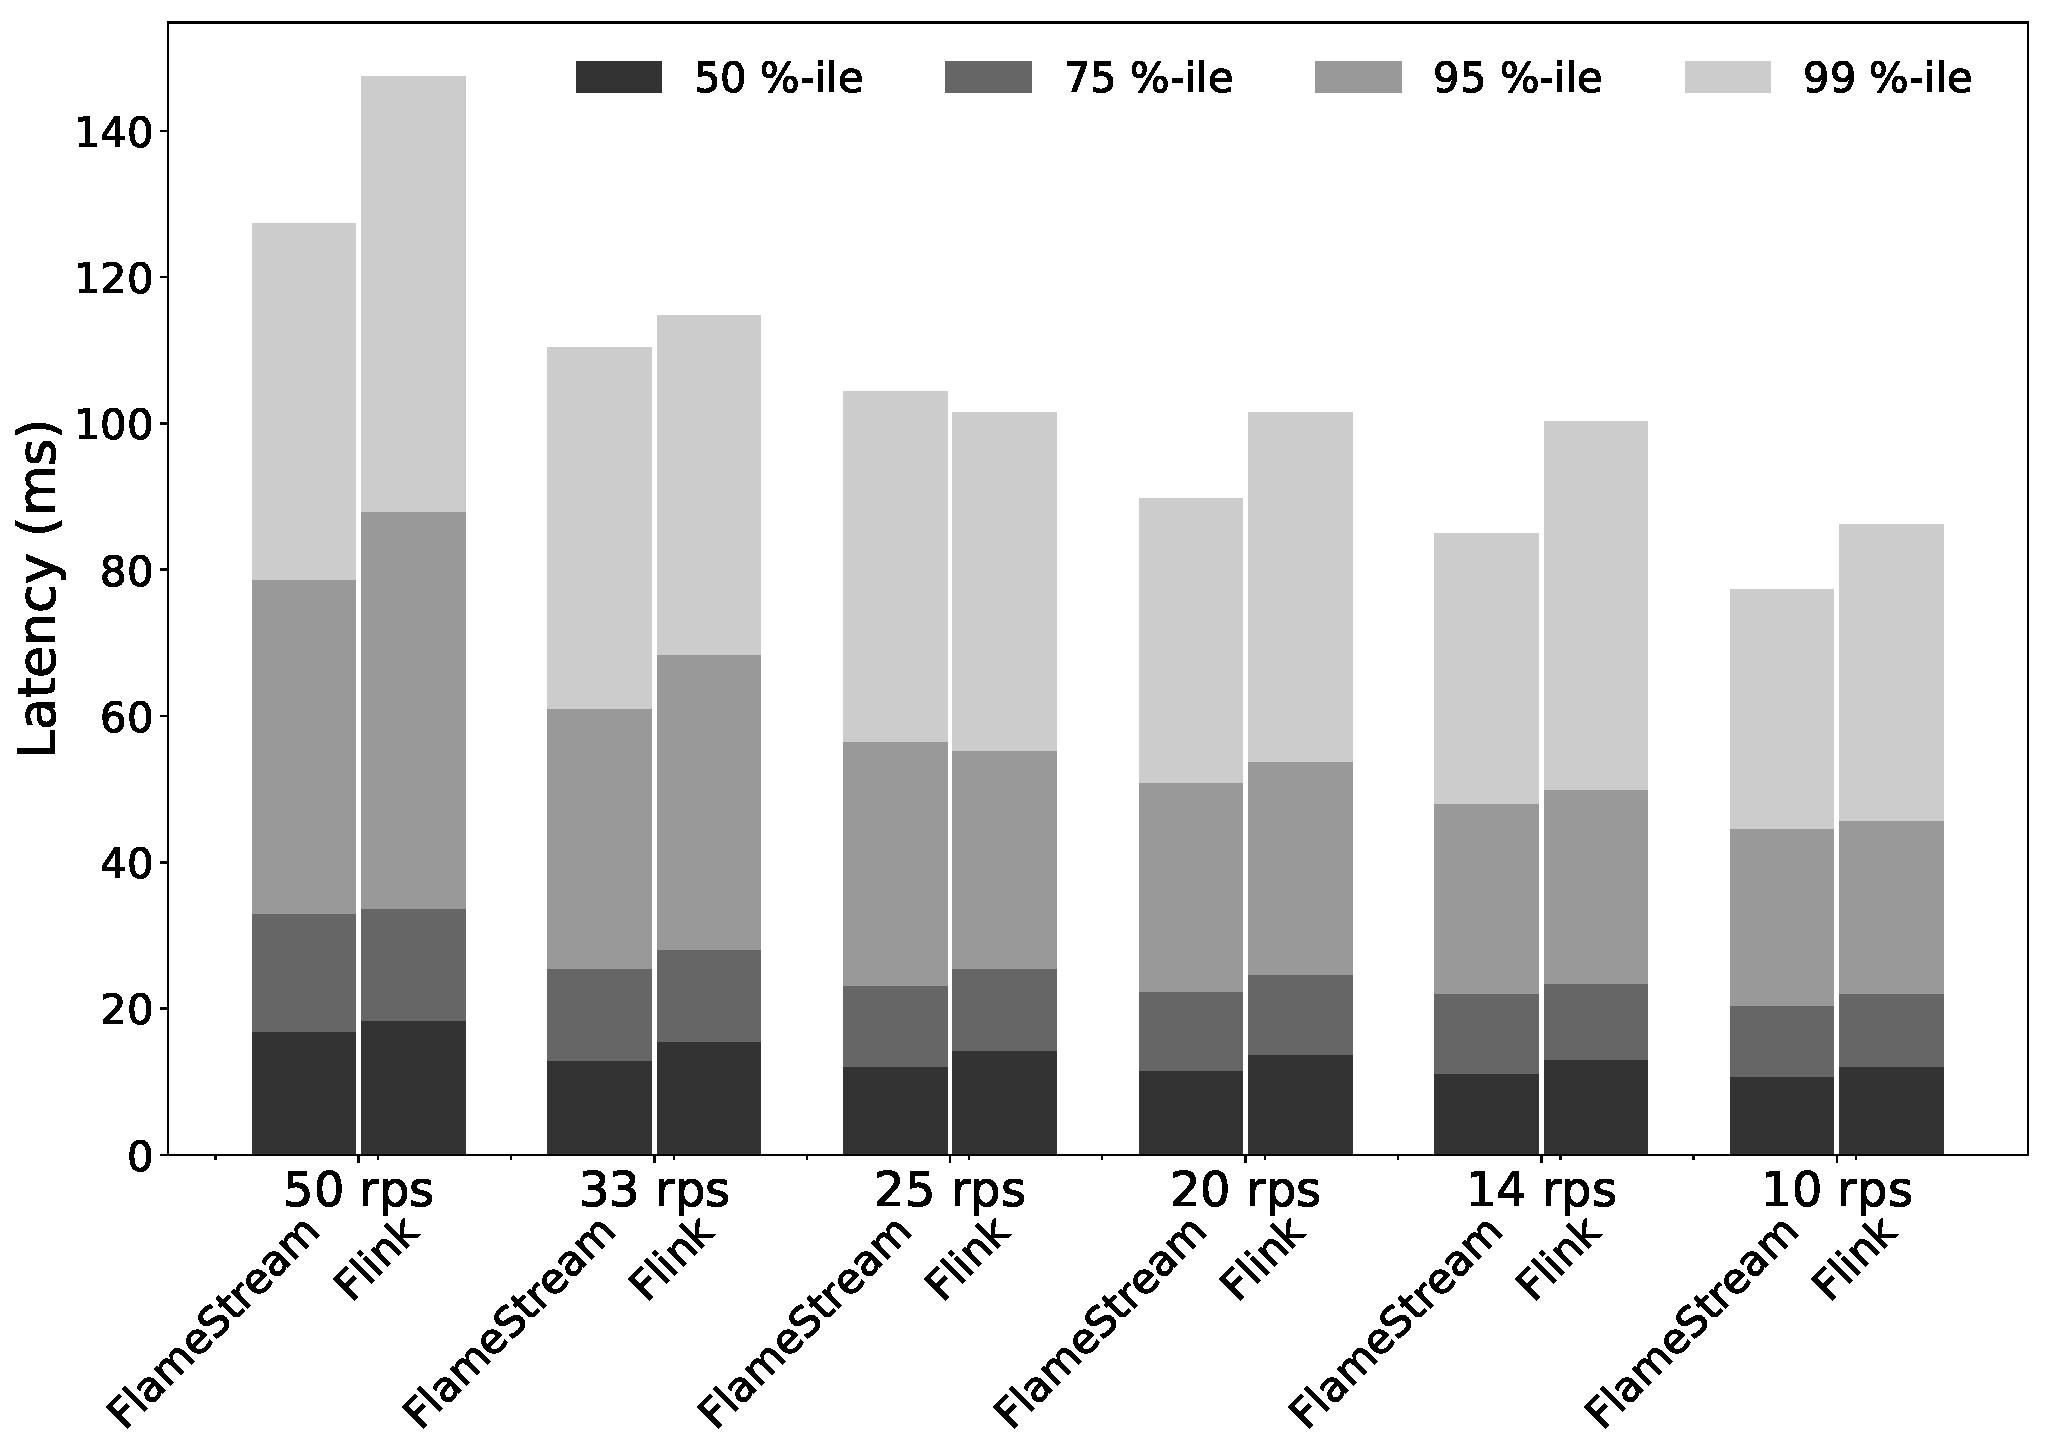
\includegraphics[width=0.5\textwidth]{pics/comp-index-quantiles}
  \caption{The comparison in latencies between \FlameStream\ and Flink within 10 nodes and distinct document rates}
  \label {fs-index-quantiles}
\end{figure}

\begin{figure}[htbp]
  \centering
  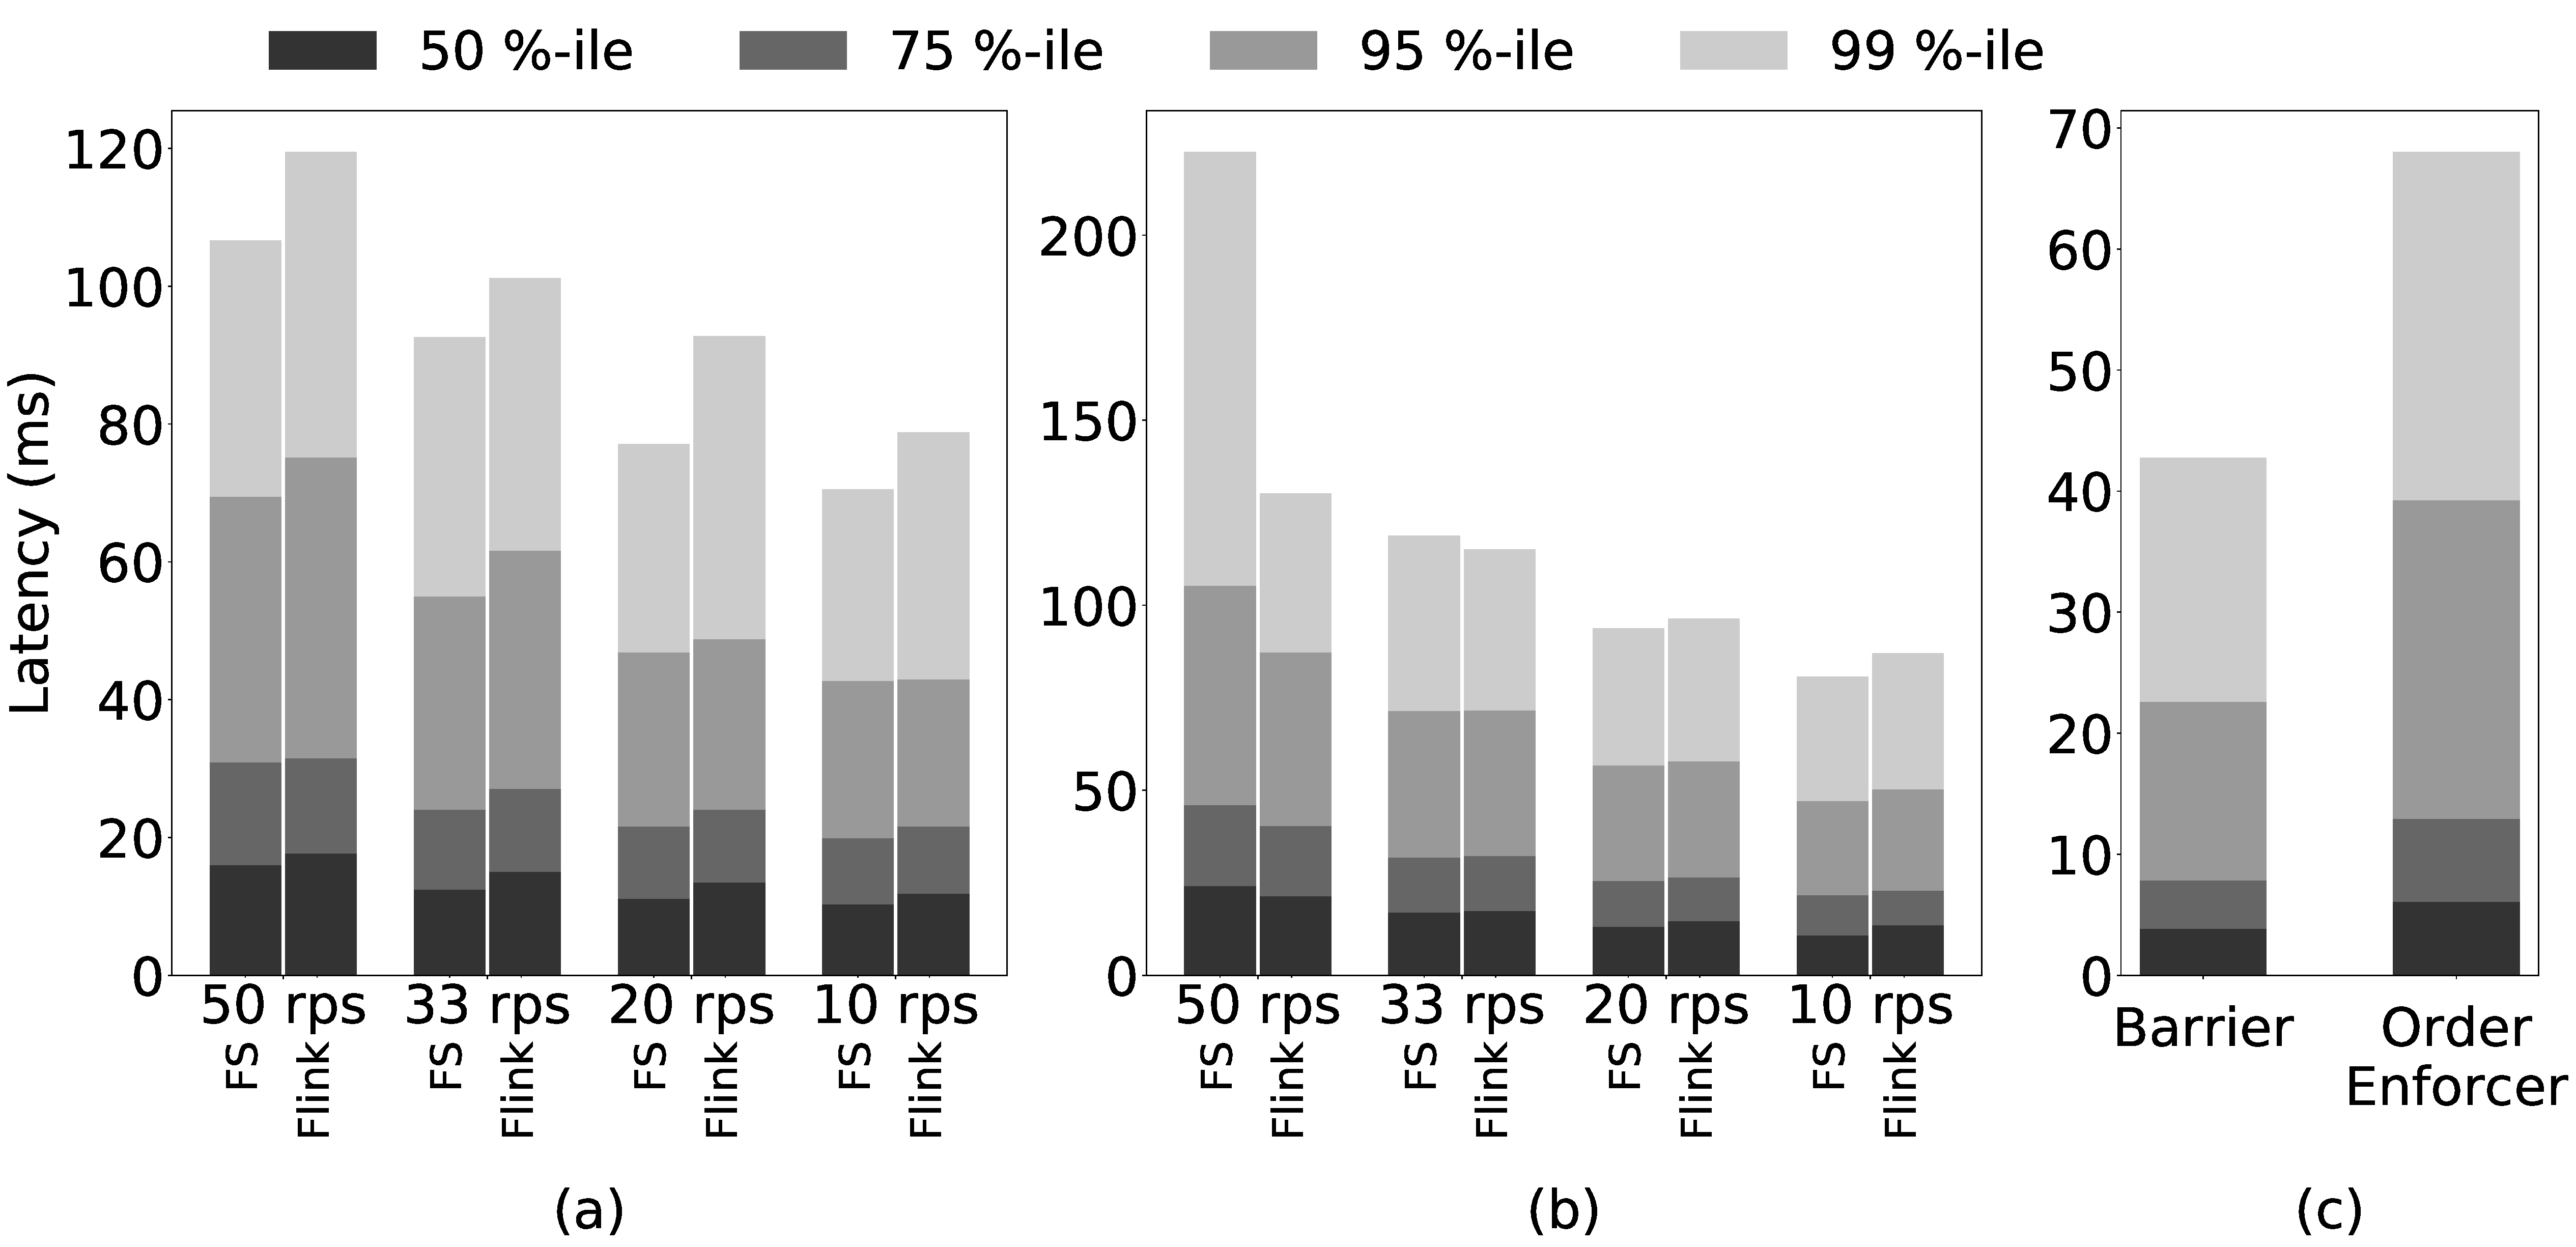
\includegraphics[width=0.25\textwidth]{pics/buffer-vs-barrier}
  \caption{Comparison between waiting time in Flink's buffer and FlameStream's barrier}
  \label {buffer-vs-barrier}
\end{figure}
